\section{Changing the position frame}
\label{sec:frames}

For a nonzero vector $v\in V$, let $C_v\le G$ be the subgroup of
permutations that preserve each pair $\{x,x+v\}$ setwise. A uniform
element of $C_v$ independently swaps or fixes each of these $n/2$
pairs with equal probability. We call it a \emph{switch in direction
$v$}.

Write $e_1,\ldots,e_d$ for the standard basis of $V$, and let
\[
 R(x_1,\ldots,x_d)=(x_2,\ldots,x_d,x_1)
\]
be left cyclic rotation. Binary strings are column vectors when a
matrix acts on them. By \eqref{eq:physical-step}, one physical
shuffle is $RS_t$, where $S_t$ is uniform in $C_{e_1}$ and the
$S_t$ are independent. Thus $Y_t=RS_tY_{t-1}$, with $Y_0=\id$.
In the rotating position frame, put
\begin{equation}\label{eq:frames:cyclic}
 X_t=R^{-t}Y_t,\qquad
 Q_t=R^{-(t-1)}S_tR^{t-1}.
\end{equation}
Then $X_t=Q_tX_{t-1}$, and the $Q_t$ are independent uniform
switches in the periodic directions
$e_1,e_2,\ldots,e_d,e_1,\ldots$. Indeed, conjugation by a linear
bijection carries $C_v$ onto the matching subgroup in the image
direction, and $R^{-(t-1)}e_1=e_{1+((t-1)\bmod d)}$.

This description also proves the finite-$d$ convergence used in
Section~\ref{sec:prelim}. A sweep of $d$ layers has positive
probability of making no swaps, and positive probability of making
exactly any chosen coordinate-edge transposition. These
transpositions generate $G$, because the cube graph is connected.
Every permutation is therefore a product of finitely many sweeps.
Padding those products by identity sweeps gives a common number of
sweeps at which every permutation has positive probability. That
kernel dominates a positive multiple of $U$, so iteration proves
convergence. The rotation is the identity at the end of each sweep.

The following path identity allows a different basis in each
successive window of $d$ directions. The maps are constructed after
the complete schedule is fixed; they need not be known when their
time index is reached.

\begin{lemma}[Fixed-schedule frame identity]
\label{lem:frames}\label{shear:lem:general-frame}
Let $T\ge d$, and let $\boldsymbol\iota=(\iota_1,\ldots,\iota_d)$
be a permutation of $1,\ldots,d$. Write
$i(t)=\iota_{1+((t-1)\bmod d)}$, and let
$X^{\boldsymbol\iota}_0=\id$ and
$X^{\boldsymbol\iota}_t=Q^{\boldsymbol\iota}_t
 X^{\boldsymbol\iota}_{t-1}$, where the increments are independent
and uniform in $C_{e_{i(t)}}$.

Fix directions $v_1,\ldots,v_T$ satisfying
\begin{equation}\label{eq:frames:bases}
 (v_s,\ldots,v_{s+d-1})\text{ is a basis of }V
 \qquad(1\le s\le T-d+1).
\end{equation}
Let $Z_0=\id$, and let $Z_t$ evolve by independent uniform switches
in these directions. There are linear bijections $L_0,\ldots,L_T$,
determined by the fixed axis order and direction schedule, such that
\begin{equation}\label{shear:eq:general-frame}
 (Z_t)_{t=0}^T\overset{\mathrm{law}}=
 \bigl(L_tX^{\boldsymbol\iota}_tL_0^{-1}\bigr)_{t=0}^T,
 \qquad L_0e_{\iota_j}=v_j\quad(1\le j\le d).
\end{equation}
In particular, if $\boldsymbol\iota=(1,\ldots,d)$ and $v_j=e_j$
for $1\le j\le d$, then $L_0=I$ and
\begin{equation}\label{eq:frames:endpoint}
 Z_T\overset{\mathrm{law}}=L_TX_T=L_TR^{-T}Y_T.
\end{equation}
\end{lemma}

\begin{proof}
For $1\le s\le T-d$, the two successive bases give unique
coefficients $a_{s,t}\in\F$, $s<t<s+d$, with
\begin{equation}\label{eq:frames:recurrence}
 v_{s+d}=v_s+\sum_{s<t<s+d}a_{s,t}v_t.
\end{equation}
The coefficient of $v_s$ cannot vanish, since otherwise
$v_{s+1},\ldots,v_{s+d}$ would be dependent; over $\F$ it is
therefore one.

We construct $L_t$ so that its column selected at time $t$ has the
required value:
\begin{equation}\label{eq:frames:selected-column}
 L_{t-1}e_{i(t)}=v_t.
\end{equation}
Begin with the map $L_0$ specified in the statement. For each time
$t$, define a row $c_t$ by putting $a_{s,t}$ in column $i(s)$
whenever $1\le s\le T-d$ and $s<t<s+d$, and putting zero in every
other column. For fixed $t$ the possible $s$ lie within at most
$d-1$ consecutive times, so their coordinate indices are distinct and
differ from $i(t)$. Thus $c_te_{i(t)}=0$. Set
\begin{equation}\label{eq:frames:matrices}
 L_t=L_{t-1}(I+e_{i(t)}c_t).
\end{equation}
Each factor squares to $I$ and is invertible. It leaves the
selected column unchanged and adds prescribed multiples of that
column to the others.

Before a column's first selection no prescribed update targets it,
so \eqref{eq:frames:selected-column} holds during the first period
by the definition of $L_0$. If it is selected at time $s$ and again
at $s+d\le T$, it has value $v_s$ after the first selection. At
each intervening time $t$ it receives $a_{s,t}$ times the selected
column, whose value is $v_t$ by induction. Equation
\eqref{eq:frames:recurrence} gives its value $v_{s+d}$ before its
next selection. This proves \eqref{eq:frames:selected-column},
including an incomplete last period.

For this fixed schedule, define the transformed step shown in
Figure~\ref{fig:frames}:
\begin{equation}\label{eq:frames:transformed-step}
 \widetilde Q_t
 =L_tQ^{\boldsymbol\iota}_tL_{t-1}^{-1}
 =(L_tL_{t-1}^{-1})
   (L_{t-1}Q^{\boldsymbol\iota}_tL_{t-1}^{-1}).
\end{equation}
In \eqref{eq:frames:transformed-step}, the second factor is uniform in
$C_{v_t}$. The first is a fixed
member of that subgroup: writing $f_t=c_tL_{t-1}^{-1}$,
\[
 L_tL_{t-1}^{-1}=I+v_tf_t,\qquad f_t(v_t)=0.
\]
The map $x\mapsto x+f_t(x)v_t$ fixes or swaps each pair
$\{x,x+v_t\}$ because $f_t$ is constant on the pair. Multiplication
by it preserves the uniform law on $C_{v_t}$. Each
$\widetilde Q_t$ depends on its own independent increment
$Q^{\boldsymbol\iota}_t$, so the transformed switches are
independent. Their products telescope at every time:
\[
 \widetilde Q_t\cdots\widetilde Q_1
 =L_tQ^{\boldsymbol\iota}_t\cdots Q^{\boldsymbol\iota}_1L_0^{-1}
 =L_tX^{\boldsymbol\iota}_tL_0^{-1}.
\]
This gives the joint path identity, and the cyclic specialization
follows from \eqref{eq:frames:cyclic}.
\end{proof}

\begin{figure}[b]
 \centering
 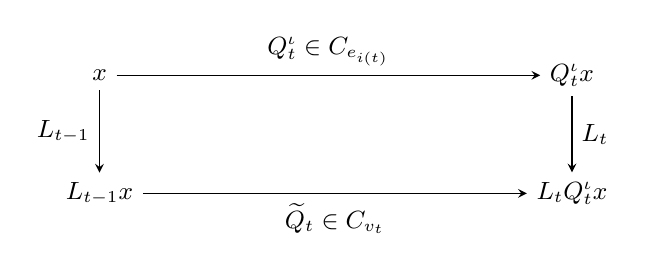
\begin{tikzpicture}[>=stealth, every node/.style={font=\small}]
  \node (a) at (0,1.5) {$x$};
  \node (b) at (6,1.5) {$Q^{\boldsymbol\iota}_tx$};
  \node (c) at (0,0) {$L_{t-1}x$};
  \node (d) at (6,0) {$L_tQ^{\boldsymbol\iota}_tx$};
  \draw[->] (a) -- node[above] {$Q^{\boldsymbol\iota}_t\in C_{e_{i(t)}}$} (b);
  \draw[->] (a) -- node[left] {$L_{t-1}$} (c);
  \draw[->] (b) -- node[right] {$L_t$} (d);
  \draw[->] (c) -- node[below] {$\widetilde Q_t\in C_{v_t}$} (d);
 \end{tikzpicture}
 \caption{One matching switch in two position frames. After the
 complete schedule is fixed, the vertical maps are deterministic
 and the lower step is an independent uniform switch in direction
 $v_t$.}
 \label{fig:frames}
\end{figure}

\begin{corollary}[Endpoint distances and the input map]
\label{cor:frames:marginals}
Under Lemma~\ref{lem:frames}, let $0\le q\le n$ and let $\pi_q$ be uniform on ordered
distinct $q$-tuples of positions. For every fixed ordered list $C$
of $q$ distinct labels,
\begin{equation}\label{eq:frames:tuple-input-map}
 \|\mathcal L(Z_T(C))-\pi_q\|_{\TV}
 =
 \|\mathcal L(X^{\boldsymbol\iota}_T(L_0^{-1}C))-\pi_q\|_{\TV}.
\end{equation}
Thus the same-list distances agree when $L_0=I$. Their averages
also agree when $C$ is sampled uniformly over ordered distinct lists,
independently of the switch process:
\begin{equation}\label{eq:frames:averaged-input-map}
 \E_C\|\mathcal L(Z_T(C)\mid C)-\pi_q\|_{\TV}
 =
 \E_C\|\mathcal L(X^{\boldsymbol\iota}_T(C)\mid C)-\pi_q\|_{\TV}.
\end{equation}
\end{corollary}
\begin{proof}
The terminal map $L_T$ is a bijection on distinct position tuples
and preserves $\pi_q$, which proves
\eqref{eq:frames:tuple-input-map}. The input map $L_0^{-1}$ also
preserves the uniform law on distinct lists, giving the averaged
identity.
\end{proof}

\begin{remark}[The schedule is fixed before the frame is constructed]
\label{rem:frames:conditioning}
If a random schedule satisfying \eqref{eq:frames:bases} is sampled
independently of the switch randomness, the lemma and corollary
apply conditionally on each complete schedule. The averaged
identity then uses a list sampled independently of that schedule
and of the switches. The maps $L_t$, including $L_0$ when the first
basis is random, may depend on directions that have not yet been
revealed. We use them only in these conditional path and endpoint
comparisons. The energy calculation next uses a separately
generated process with directions revealed in chronological order.
\end{remark}
